\documentclass[11pt]{article}   % tipo de documento e tamanho das letras

% os seguintes pacotes estendem a funcionalidade básica:
\usepackage[a4paper, total={16cm, 24cm}]{geometry} % tamanho da pagina e do texto
\usepackage[portuguese]{babel}  % traduz para portugues
\usepackage[utf8]{inputenc}
\usepackage{graphicx}           % graficos
\usepackage{amsmath}            % matematica
\usepackage{tikz}               % diagramas
    \usetikzlibrary{shadows}
\usepackage{booktabs}           % tabelas com  melhor aspecto
\usepackage[colorlinks=true]{hyperref}           % links para partes do documento ou para a web
\usepackage{listings}           % incluir codigo
    \renewcommand\lstlistingname{Listagem}  % Listing em portugues
    \lstset{numbers=left, numberstyle=\tiny, numbersep=5pt, basicstyle=\footnotesize\ttfamily, frame=tb,rulesepcolor=\color{gray}, breaklines=true}
\usepackage{blindtext}

% -------------------------------------------------------------------------------------------
\title
{
    
\includegraphics[width=0.3\textwidth]{images/logo_universidade.png}
    \\[0.1cm]
    \textbf{Gerador de Árvores de Decisão} \\
    Aprendizagem Automática
}

\author
{
    \textbf{Professores:} Teresa Gonçalves \\ Luís Rato \\
    \textbf{Realizado por:} Miguel de Carvalho (43108) \\ João Pereira (42864) 
}
\date{\today}

% -------------------------------------------------------------------------------------------
%                                Body                                                       %
% -------------------------------------------------------------------------------------------

\begin{document}
\maketitle

% -------------------------------------------------------------------------------------------
\section{Introdução} 

\hspace{0,5cm}Neste trabalho foi solicitado a realização de um programa que simule a criação de \textbf{Árvores de Decisão} com \textbf{pruning}, 
representado na figura abaixo. \par
\begin{figure}[h!]
    \begin{center}
	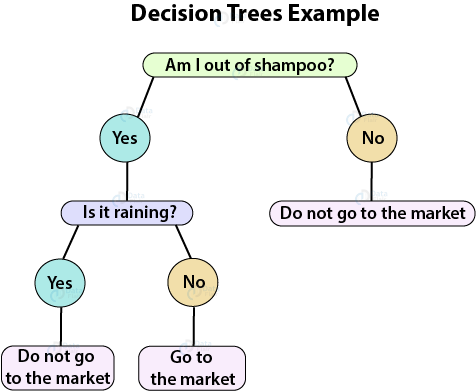
\includegraphics[width=0.5\textwidth]{images/tree-example.png}
        \caption{Exemplo de uma Árvore de Decisão}
    \end{center}
\end{figure}
A \textbf{Árvore de Decisão} é uma forma expressiva e fácil de perceber como será feita a decisão para os dados em questão.


É constituída por:
\begin{itemize}
    \item \textbf{Nós (Nodes)} são as perguntas feitas para ser tomada uma decisão, por conseguinte a decisão irá escolher por qual \textbf{ramo} vai passar;
    \item \textbf{Ramos (Branchs)} são as decisões que são tomadas, que vão levar a outro \textbf{nó} ou mesmo a uma \textbf{folha};
    \item \textbf{Folhas (Leafs)} é a \textbf{classe} (resposta final) que corresponde à(s) decisão(ões).
\end{itemize}
\begin{figure}[h!]
    \begin{center}
	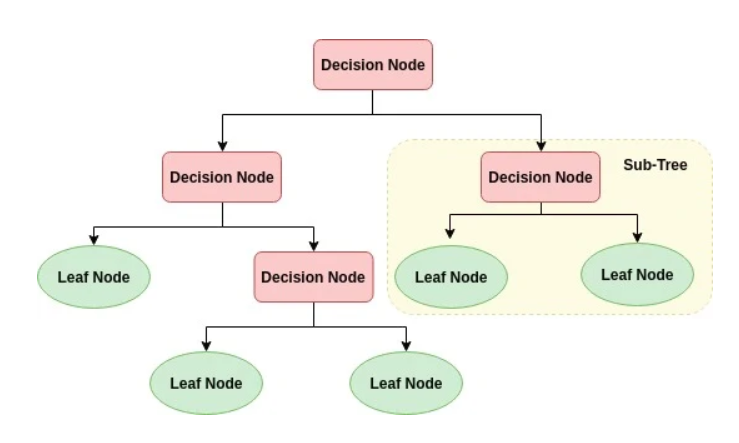
\includegraphics[width=0.5\textwidth]{images/tree-structure.png}
        \caption{Estrutura de uma Árvore de Decisão}
    \end{center}
\end{figure}


Existem vários \textbf{critérios} para realizar a decisão de qual deverá ser o \textbf{nó} escolhido, ou seja,
qual deverá ser a melhor questão a ser feita em cada instante. \par
Neste trabalho serão utilizados o seguintes critérios \textbf{Entropia}, \textbf{Gini} e o \textbf{Erro}:
\begin{itemize}
    \item A \textbf{Entropia} é a informação esperada em bits;
    \item O \textbf{Gini} é o erro esperado se etiquetar as folhas aleatoriamente; 
    \item O \textbf{Erro} é também conhecido como razão do erro.
\end{itemize}

% -------------------------------------------------------------------------------------------
\section{Implementação}

% -------------------------------------------------------------------------------------------
\section{Funções}
% -------------------------------------------------------------------------------------------
\section{Execução}

% -------------------------------------------------------------------------------------------
\section{Análise de Resultados}
% -------------------------------------------------------------------------------------------
\newpage
\section{Conclusão} % Conclusão
\hspace{0,5cm}Em suma, com a realização deste trabalho "Gerador de Árvores de Decisão" fiquei muito mais esclarecido sobre o seu funcionamento. \par
Saliento que me ajudou a entender como funciona o escalonador e as condições que cada algoritmo (\textbf{FCFS}/\textbf{RR}), usa para proceder à mudança dos processos entre os estados e as respetivas diferenças de tempo no mesmo conjunto de processos, entre os respetivos algoritmos.  
% -------------------------------------------------------------------------------------------
\end{document}
